% Options for packages loaded elsewhere
\PassOptionsToPackage{unicode}{hyperref}
\PassOptionsToPackage{hyphens}{url}
%
\documentclass[
]{book}
\usepackage{amsmath,amssymb}
\usepackage{lmodern}
\usepackage{ifxetex,ifluatex}
\ifnum 0\ifxetex 1\fi\ifluatex 1\fi=0 % if pdftex
  \usepackage[T1]{fontenc}
  \usepackage[utf8]{inputenc}
  \usepackage{textcomp} % provide euro and other symbols
\else % if luatex or xetex
  \usepackage{unicode-math}
  \defaultfontfeatures{Scale=MatchLowercase}
  \defaultfontfeatures[\rmfamily]{Ligatures=TeX,Scale=1}
\fi
% Use upquote if available, for straight quotes in verbatim environments
\IfFileExists{upquote.sty}{\usepackage{upquote}}{}
\IfFileExists{microtype.sty}{% use microtype if available
  \usepackage[]{microtype}
  \UseMicrotypeSet[protrusion]{basicmath} % disable protrusion for tt fonts
}{}
\makeatletter
\@ifundefined{KOMAClassName}{% if non-KOMA class
  \IfFileExists{parskip.sty}{%
    \usepackage{parskip}
  }{% else
    \setlength{\parindent}{0pt}
    \setlength{\parskip}{6pt plus 2pt minus 1pt}}
}{% if KOMA class
  \KOMAoptions{parskip=half}}
\makeatother
\usepackage{xcolor}
\IfFileExists{xurl.sty}{\usepackage{xurl}}{} % add URL line breaks if available
\IfFileExists{bookmark.sty}{\usepackage{bookmark}}{\usepackage{hyperref}}
\hypersetup{
  pdftitle={A New Instrument for Microbial Epidemiology},
  pdfauthor={Matthijs S. Berends},
  hidelinks,
  pdfcreator={LaTeX via pandoc}}
\urlstyle{same} % disable monospaced font for URLs
\usepackage{color}
\usepackage{fancyvrb}
\newcommand{\VerbBar}{|}
\newcommand{\VERB}{\Verb[commandchars=\\\{\}]}
\DefineVerbatimEnvironment{Highlighting}{Verbatim}{commandchars=\\\{\}}
% Add ',fontsize=\small' for more characters per line
\usepackage{framed}
\definecolor{shadecolor}{RGB}{248,248,248}
\newenvironment{Shaded}{\begin{snugshade}}{\end{snugshade}}
\newcommand{\AlertTok}[1]{\textcolor[rgb]{0.94,0.16,0.16}{#1}}
\newcommand{\AnnotationTok}[1]{\textcolor[rgb]{0.56,0.35,0.01}{\textbf{\textit{#1}}}}
\newcommand{\AttributeTok}[1]{\textcolor[rgb]{0.77,0.63,0.00}{#1}}
\newcommand{\BaseNTok}[1]{\textcolor[rgb]{0.00,0.00,0.81}{#1}}
\newcommand{\BuiltInTok}[1]{#1}
\newcommand{\CharTok}[1]{\textcolor[rgb]{0.31,0.60,0.02}{#1}}
\newcommand{\CommentTok}[1]{\textcolor[rgb]{0.56,0.35,0.01}{\textit{#1}}}
\newcommand{\CommentVarTok}[1]{\textcolor[rgb]{0.56,0.35,0.01}{\textbf{\textit{#1}}}}
\newcommand{\ConstantTok}[1]{\textcolor[rgb]{0.00,0.00,0.00}{#1}}
\newcommand{\ControlFlowTok}[1]{\textcolor[rgb]{0.13,0.29,0.53}{\textbf{#1}}}
\newcommand{\DataTypeTok}[1]{\textcolor[rgb]{0.13,0.29,0.53}{#1}}
\newcommand{\DecValTok}[1]{\textcolor[rgb]{0.00,0.00,0.81}{#1}}
\newcommand{\DocumentationTok}[1]{\textcolor[rgb]{0.56,0.35,0.01}{\textbf{\textit{#1}}}}
\newcommand{\ErrorTok}[1]{\textcolor[rgb]{0.64,0.00,0.00}{\textbf{#1}}}
\newcommand{\ExtensionTok}[1]{#1}
\newcommand{\FloatTok}[1]{\textcolor[rgb]{0.00,0.00,0.81}{#1}}
\newcommand{\FunctionTok}[1]{\textcolor[rgb]{0.00,0.00,0.00}{#1}}
\newcommand{\ImportTok}[1]{#1}
\newcommand{\InformationTok}[1]{\textcolor[rgb]{0.56,0.35,0.01}{\textbf{\textit{#1}}}}
\newcommand{\KeywordTok}[1]{\textcolor[rgb]{0.13,0.29,0.53}{\textbf{#1}}}
\newcommand{\NormalTok}[1]{#1}
\newcommand{\OperatorTok}[1]{\textcolor[rgb]{0.81,0.36,0.00}{\textbf{#1}}}
\newcommand{\OtherTok}[1]{\textcolor[rgb]{0.56,0.35,0.01}{#1}}
\newcommand{\PreprocessorTok}[1]{\textcolor[rgb]{0.56,0.35,0.01}{\textit{#1}}}
\newcommand{\RegionMarkerTok}[1]{#1}
\newcommand{\SpecialCharTok}[1]{\textcolor[rgb]{0.00,0.00,0.00}{#1}}
\newcommand{\SpecialStringTok}[1]{\textcolor[rgb]{0.31,0.60,0.02}{#1}}
\newcommand{\StringTok}[1]{\textcolor[rgb]{0.31,0.60,0.02}{#1}}
\newcommand{\VariableTok}[1]{\textcolor[rgb]{0.00,0.00,0.00}{#1}}
\newcommand{\VerbatimStringTok}[1]{\textcolor[rgb]{0.31,0.60,0.02}{#1}}
\newcommand{\WarningTok}[1]{\textcolor[rgb]{0.56,0.35,0.01}{\textbf{\textit{#1}}}}
\usepackage{longtable,booktabs,array}
\usepackage{calc} % for calculating minipage widths
% Correct order of tables after \paragraph or \subparagraph
\usepackage{etoolbox}
\makeatletter
\patchcmd\longtable{\par}{\if@noskipsec\mbox{}\fi\par}{}{}
\makeatother
% Allow footnotes in longtable head/foot
\IfFileExists{footnotehyper.sty}{\usepackage{footnotehyper}}{\usepackage{footnote}}
\makesavenoteenv{longtable}
\usepackage{graphicx}
\makeatletter
\def\maxwidth{\ifdim\Gin@nat@width>\linewidth\linewidth\else\Gin@nat@width\fi}
\def\maxheight{\ifdim\Gin@nat@height>\textheight\textheight\else\Gin@nat@height\fi}
\makeatother
% Scale images if necessary, so that they will not overflow the page
% margins by default, and it is still possible to overwrite the defaults
% using explicit options in \includegraphics[width, height, ...]{}
\setkeys{Gin}{width=\maxwidth,height=\maxheight,keepaspectratio}
% Set default figure placement to htbp
\makeatletter
\def\fps@figure{htbp}
\makeatother
\setlength{\emergencystretch}{3em} % prevent overfull lines
\providecommand{\tightlist}{%
  \setlength{\itemsep}{0pt}\setlength{\parskip}{0pt}}
\setcounter{secnumdepth}{5}
\usepackage{booktabs}
\usepackage{amsthm}
\makeatletter
\def\thm@space@setup{%
  \thm@preskip=8pt plus 2pt minus 4pt
  \thm@postskip=\thm@preskip
}
\makeatother
\ifluatex
  \usepackage{selnolig}  % disable illegal ligatures
\fi
\usepackage[]{natbib}
\bibliographystyle{apalike}

\title{A New Instrument for Microbial Epidemiology}
\usepackage{etoolbox}
\makeatletter
\providecommand{\subtitle}[1]{% add subtitle to \maketitle
  \apptocmd{\@title}{\par {\large #1 \par}}{}{}
}
\makeatother
\subtitle{Empowering Antimicrobial Resistance Data Analysis}
\author{Matthijs S. Berends}
\date{}

\begin{document}
\maketitle

{
\setcounter{tocdepth}{1}
\tableofcontents
}
\hypertarget{preamble}{%
\chapter*{Preamble}\label{preamble}}
\addcontentsline{toc}{chapter}{Preamble}

This is the integral PhD thesis `A New Instrument for Microbial Epidemiology' (DOI \href{https://doi.org/10.33612/diss.177417131}{10.33612/diss.177417131}) by \href{https://www.rug.nl/staff/m.s.berends}{Matthijs S. Berends}, which was defended publicly at the University of Groningen, the Netherlands, on 25 August 2021.

All texts were copied from the printed version `as is'; no modifications were made.

\hypertarget{short-summary-250-words}{%
\subsection*{Short summary (250 words)}\label{short-summary-250-words}}
\addcontentsline{toc}{subsection}{Short summary (250 words)}

Treating infectious diseases requires insights into the microorganisms causing infectious diseases. Antimicrobial resistance (AMR) in microorganisms limits treatment possibilities and poses an enormous healthcare problem worldwide. The spread and AMR patterns of microorganisms, risk factors for infection, and preventive and control measures of infectious disease are studied within the field of Microbial Epidemiology, a cross-over field between Epidemiology and Clinical Microbiology. For analysing the spread and AMR patterns of microorganisms, however, no standardised method previously existed. This thesis showcases the development and applied use of a new instrument to analyse AMR data: the AMR package for R. From multiple viewpoints, the AMR package and its advantages are put into perspective: from a technical viewpoint, from an infection management viewpoint and from a clinical viewpoint. These combined provide a common ground for comprehending what the AMR package could yield in the field and how it can set a new empowered starting point for future applications of microbial epidemiology, in clinical and research settings alike. This thesis subsequently elaborates on these multiple viewpoints by illustrating the use of this new instrument in epidemiological research projects in the Dutch-German cross-border region to better understand the occurrence and AMR patterns of microorganisms on a (eu)regional level. In conclusion, this thesis shows the added value of a consistent data-analytical instrument to prepare and analyse AMR data in a full-region approach, that can also be used in clinical settings to obtain novel insights on AMR patterns.

\hypertarget{colophon}{%
\chapter*{Colophon}\label{colophon}}
\addcontentsline{toc}{chapter}{Colophon}

Cover design: Matthijs Berends (images used with permission)\\
Layout: Matthijs Berends\\
Printing: Gildeprint -- www.gildeprint.nl

The work described within this thesis was supported by (1) the Certe Medical Diagnostics and Advice Foundation, (2) the INTERREG V A (202085) funded project EurHealth-1Health (\url{http://www.eurhealth1health.eu}), part of a Dutch-German cross-border network supported by the European Commission, the Dutch Ministry of Health, Welfare and Sport, the Ministry of Economy, Innovation, Digitalisation and Energy of the German Federal State of North Rhine-Westphalia, and the Ministry for National and European Affairs and Regional Development of the German Federal State of Lower Saxony, (3) the European Union's Horizon 2020 Research and Innovation Programme under the Marie Skłodowska-Curie Grant Agreement 713660 (MSCA-COFUND-2015-DP ``Pronkjewail''), and (4) the European Society for Clinical Microbiology and Infectious Diseases (ESCMID) through the ESCMID Study Group for Antimicrobial Stewardship (ESGAP).

Printing of this thesis was financially supported by the Certe Medical Diagnostics and Advice Foundation. This support is greatly appreciated.

\textbf{Copyright © 2021 by Matthias Simeon Berends.} All rights reserved. Any unauthorised reprint or use of this material is prohibited. No parts of this thesis may be reproduced, stored, or transmitted in any form or by any means, without written permission of the author or, when appropriate, the publishers of the publications.

\hypertarget{introduction}{%
\chapter{Introduction}\label{introduction}}

\hypertarget{microbial-epidemiology}{%
\section{Microbial Epidemiology}\label{microbial-epidemiology}}

Epidemiology is the medical scientific field that investigates all the factors that determine the presence or absence of diseases and disorders. While many subspecialties within this field exist nowadays, such as veterinary epidemiology and cardiovascular epidemiology, its development started with an infectious disease. Between 1846 and 1860, the world endured the third cholera pandemic, taking assumably millions of lives \textsuperscript{{[}1{]}}. The year 1854 was considered the worst year, when 23,000 people died in the United Kingdom, out of 16 million inhabitants (0.14\%) \textsuperscript{{[}2{]}}. As a side note, this is still quite less than the 146,000 UK deaths due to COVID-19 out of 56 million inhabitants (0.26\%) until March 2021 \textsuperscript{{[}3{]}}. But 1854 was also the year that the basis was laid for the field of epidemiology by John Snow, an English physician and hygiene specialist.

At the time of a local cholera outbreak at the Broad Street in London in that year, Snow did not know the exact source of cholera and called it `cholera poison' in a book he published in 1856 \textsuperscript{{[}4{]}}. Interestingly, the Italian Filippo Pacini managed to isolate the bacterium causing cholera, \emph{Vibrio cholerae}, in 1854 -- the same year that Snow investigated the outbreak \textsuperscript{{[}5{]}}. Although it was not until 1884 that \emph{V. cholerae} was formally given its name by the German Robert Koch \textsuperscript{{[}6{]}}.

In his book about the `cholera poison', Snow famously wrote \textsuperscript{{[}4{]}}:

\begin{quote}
``There is no doubt that the mortality was much diminished, as I said before, by the flight of the population, which commenced soon after the outbreak; but the attacks had so far diminished before the use of the water was stopped, that it is impossible to decide whether the well still contained the cholera poison in an active state, or whether, from some cause, the water had become free from it.''
\end{quote}

\hypertarget{references}{%
\section*{References}\label{references}}
\addcontentsline{toc}{section}{References}

{[}1{]} Hays JN. Epidemics and pandemics: their impacts on human history. Santa Barbara, Calif.; 2005.
{[}2{]} Paneth N, Vinten-Johansen P, Brody H, Rip M. A rivalry of foulness: official and unofficial investigations of the London cholera epidemic of 1854. Am J Public Health 1998;88:1545--53. \url{doi:10.2105/AJPH.88.10.1545}.
{[}3{]} Office for National Statistics. Deaths with COVID-19 on the death certificate. 5 March 2021 2021. \url{https://coronavirus.data.gov.uk/details/deaths} (accessed March 21, 2021).
{[}4{]} Snow J. On the Mode of Communication of Cholera. Edinb Med J 1856;1:668--70.
{[}5{]} Pacini F. Osservazioni microscopiche e deduzioni patologiche sul cholera asiatico. Gazz Medica Ital Toscana 1854;4:397--401.
{[}6{]} Howard-Jones N. Robert Koch and the cholera vibrio: a centenary. BMJ 1984;288:379--81. \url{doi:10.1136/bmj.288.6414.379}.
{[}7{]} World Health Organization. Antimicrobial resistance Fact sheet N°194. April 2014 2014. \url{https://www.who.int/mediacentre/factsheets/fs194/en/} (accessed March 21, 2021).
{[}8{]} O'Neill J. Antimicrobial Resistance: Tackling a Crisis for the Health and Wealth of Nations.
Rev Antimicrob Resist 2014:1--16.
{[}9{]} de Kraker MEA, Stewardson AJ, Harbarth S. Will 10 Million People Die a Year due to Antimicrobial Resistance by 2050? PLOS Med 2016;13:e1002184. \url{doi:10.1371/journal.pmed.1002184}.

You can label chapter and section titles using \texttt{\{\#label\}} after them, e.g., we can reference Chapter \ref{introduction}.

Figures and tables with captions will be placed in \texttt{figure} and \texttt{table} environments, respectively.

\begin{Shaded}
\begin{Highlighting}[]
\FunctionTok{par}\NormalTok{(}\AttributeTok{mar =} \FunctionTok{c}\NormalTok{(}\DecValTok{4}\NormalTok{, }\DecValTok{4}\NormalTok{, .}\DecValTok{1}\NormalTok{, .}\DecValTok{1}\NormalTok{))}
\FunctionTok{plot}\NormalTok{(pressure, }\AttributeTok{type =} \StringTok{\textquotesingle{}b\textquotesingle{}}\NormalTok{, }\AttributeTok{pch =} \DecValTok{19}\NormalTok{)}
\end{Highlighting}
\end{Shaded}

\begin{figure}

{\centering 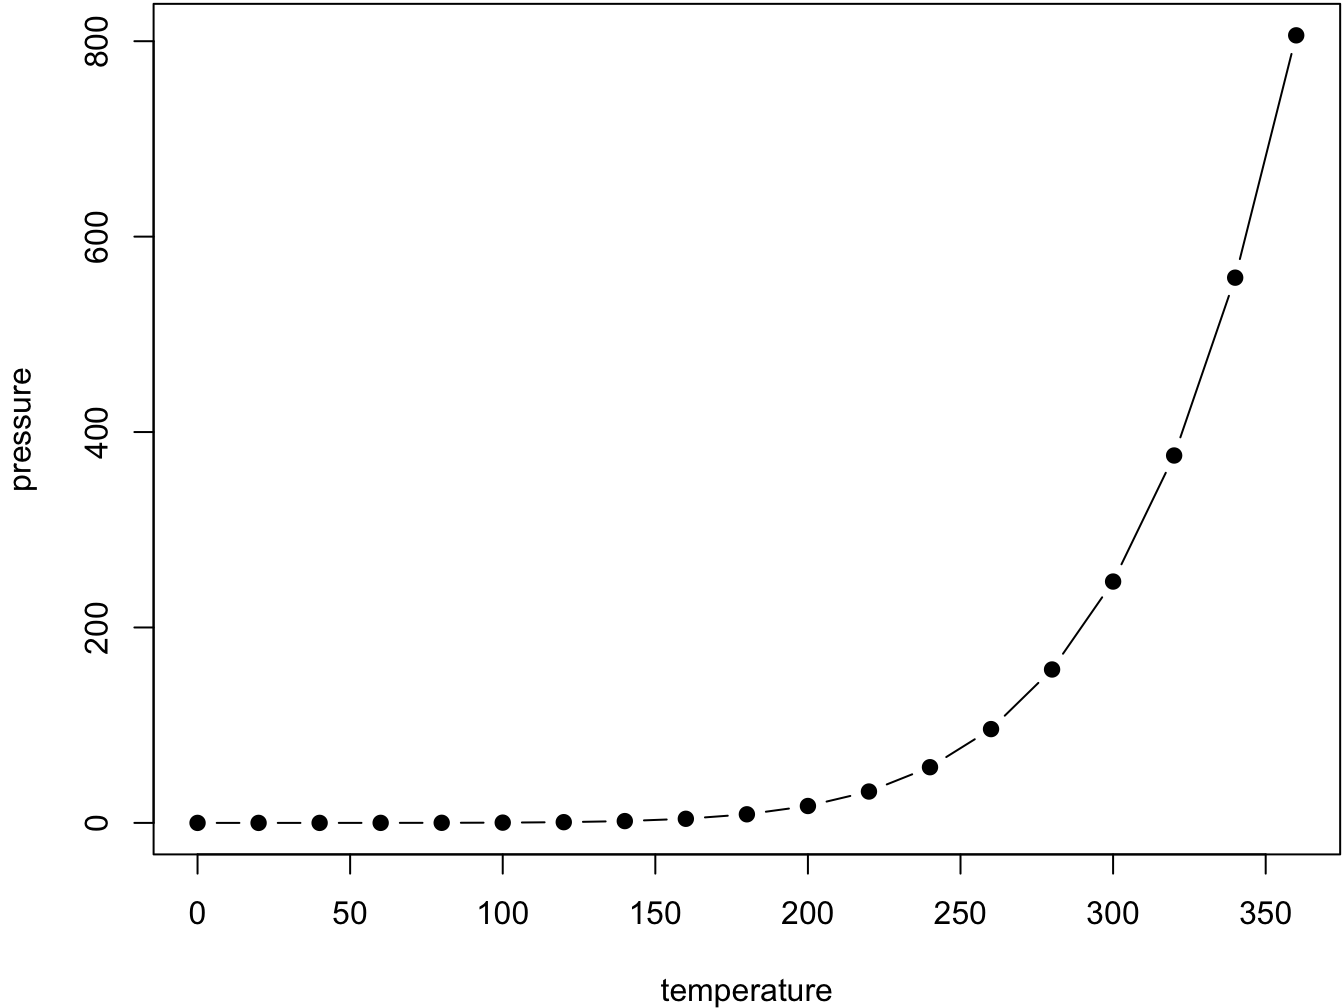
\includegraphics[width=0.8\linewidth]{a_new_instrument_for_microbial_epidemiology_files/figure-latex/nice-fig-1} 

}

\caption{Here is a nice figure!}\label{fig:nice-fig}
\end{figure}

Reference a figure by its code chunk label with the \texttt{fig:} prefix, e.g., see Figure \ref{fig:nice-fig}. Similarly, you can reference tables generated from \texttt{knitr::kable()}, e.g., see Table \ref{tab:nice-tab}.

\begin{Shaded}
\begin{Highlighting}[]
\NormalTok{knitr}\SpecialCharTok{::}\FunctionTok{kable}\NormalTok{(}
  \FunctionTok{head}\NormalTok{(iris, }\DecValTok{20}\NormalTok{), }\AttributeTok{caption =} \StringTok{\textquotesingle{}Here is a nice table!\textquotesingle{}}\NormalTok{,}
  \AttributeTok{booktabs =} \ConstantTok{TRUE}
\NormalTok{)}
\end{Highlighting}
\end{Shaded}

\begin{table}

\caption{\label{tab:nice-tab}Here is a nice table!}
\centering
\begin{tabular}[t]{rrrrl}
\toprule
Sepal.Length & Sepal.Width & Petal.Length & Petal.Width & Species\\
\midrule
5.1 & 3.5 & 1.4 & 0.2 & setosa\\
4.9 & 3.0 & 1.4 & 0.2 & setosa\\
4.7 & 3.2 & 1.3 & 0.2 & setosa\\
4.6 & 3.1 & 1.5 & 0.2 & setosa\\
5.0 & 3.6 & 1.4 & 0.2 & setosa\\
\addlinespace
5.4 & 3.9 & 1.7 & 0.4 & setosa\\
4.6 & 3.4 & 1.4 & 0.3 & setosa\\
5.0 & 3.4 & 1.5 & 0.2 & setosa\\
4.4 & 2.9 & 1.4 & 0.2 & setosa\\
4.9 & 3.1 & 1.5 & 0.1 & setosa\\
\addlinespace
5.4 & 3.7 & 1.5 & 0.2 & setosa\\
4.8 & 3.4 & 1.6 & 0.2 & setosa\\
4.8 & 3.0 & 1.4 & 0.1 & setosa\\
4.3 & 3.0 & 1.1 & 0.1 & setosa\\
5.8 & 4.0 & 1.2 & 0.2 & setosa\\
\addlinespace
5.7 & 4.4 & 1.5 & 0.4 & setosa\\
5.4 & 3.9 & 1.3 & 0.4 & setosa\\
5.1 & 3.5 & 1.4 & 0.3 & setosa\\
5.7 & 3.8 & 1.7 & 0.3 & setosa\\
5.1 & 3.8 & 1.5 & 0.3 & setosa\\
\bottomrule
\end{tabular}
\end{table}

  \bibliography{packages.bib}

\end{document}
